\documentclass{article}

\usepackage[english, russian]{babel}
\usepackage{geometry}
\usepackage{graphicx}
\usepackage{listings}
\usepackage{xcolor}
\usepackage[12pt]{extsizes}
\usepackage{amsmath}
\usepackage{setspace}
\usepackage{multirow}
\usepackage{tocloft}
\usepackage{indentfirst} 
\usepackage{lipsum}
\usepackage{caption}
\usepackage{cmap}
\usepackage[utf8]{inputenc}
\usepackage[T2A]{fontenc}
\usepackage{titlesec}

\captionsetup[figure]{name={Рисунок},labelsep=endash}
\captionsetup[table]{singlelinecheck=false, labelsep=endash}

\setcounter{secnumdepth}{0}

\renewcommand{\cftsecleader}{\cftdotfill{\cftdotsep}}
\geometry{pdftex, left = 1cm, right = 1cm	, top = 1cm, bottom = 1cm}
\onehalfspacing

\setlength{\parindent}{1,25cm}

\pagestyle{empty}

\begin{document}

\section{\begin{center}Задача оптимизации в программировании\end{center}}
\vspace{-1cm}
Задача оптимизации в программировании -- это задача нахождения экстремума (минимума или максимума) целевой функции в 
некоторой области конечномерного векторного пространства, ограниченной набором линейных и/или нелинейных равенств или 
неравенств.$^{[1]}$


\section{\begin{center}Методы оптимизации второго порядка\end{center}}
\vspace{-1cm}
Методы оптимизации второго порядка -- это алгоритмы, которые используют информацию о вторых производных функции 
потерь для более быстрого и точного нахождения точек минимума с очень неровным и сложным ландшафтом потерь.$^{[2]}$

Один из методов оптимизации второго порядка -- это метод Ньютона$^{[3]}$ (формула \ref{formula}).
\begin{equation}
	\label{formula}
	X_{k+1} = X_k - \frac{f'(X_k)}{f''(X_k)}
\end{equation}

Метод Ньютона рекомендуется к применению в том случае, когда задача минимизации достаточно хорошо локализована. 
Схема соответствующего алгоритма приведена на рисунке \ref{img}.

\begin{figure}[h]
	\centering
	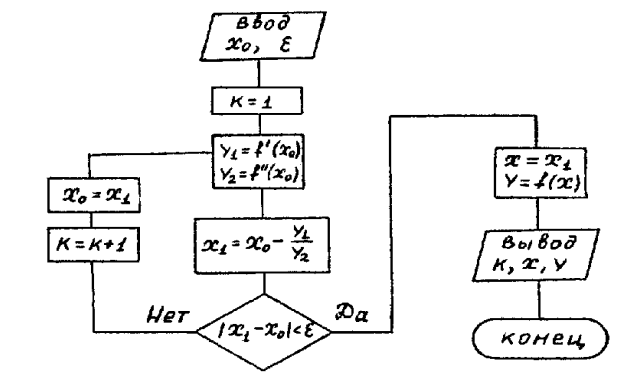
\includegraphics[scale=0.6]{img.png}
	\caption{Схема алгоритма вычисления сходимости методом Нютона}
	\label{img}
\end{figure}


\section{\begin{center}Список использованных источников\end{center}}
\vspace{-1cm}
\begin{enumerate}
	\item Suman Kalyan Adari, Sridhar Alla -- Beginning Anomaly Detection Using Python-Based Deep Learning
	\item Neal Parikh, Stephen Boyd -- Proximal Algorithms
	\item	Rohan Anil, Vineet Gupta, Tomer Koren, Kevin Regan, Yoram Singer -- Scalable Second Order Optimization for Deep Learning
\end{enumerate}

\end{document}